
\section{Misconceptions in Some Existing Results}
\subsection{Incorrect Assumptions in Critical Instant Theorem with Synchronous Releases}
\label{sec:wrong-critical}

Over the years, it has been well accepted that the characterization of the critical instant for self-suspending tasks is a complex problem. Nevertheless, although the complexity of verifying the existence of a feasible schedule for segmented self-suspending tasks has been proven to be ${\cal NP}$-hard in the strong sense \cite{Ridouard_2004}, the complexity of verifying the schedulability of a task set has only been studied for segmented self-suspending tasks with constrained deadlines scheduled with a dynamic priority scheduling algorithm (see Section~\ref{sec:hardness}), hence leaving hope for the existence efficient schedulability tests for more constrained systems. 

Following that idea, Lakshmanan and Rajkumar proposed a pseudo-polynomial worst-case response time analysis for one segmented self-suspending task $\tau_i$ assuming that 
\begin{itemize}
\item the scheduling algorithm is fixed priority (FP);
\item $\tau_i$ is the lowest priority task; 
\item all the higher priority tasks are sporadic;
\item all the higher priority tasks are non-self-suspending.
\end{itemize}
The analysis, presented \cite{RTAS-LakshmananR10}, is based on the notion of critical instant, i.e., an instant at which, considering the state of the system, an execution request for $\tau_i$ will generate the largest response time. This critical instant was defined as follows:
\begin{itemize}
	\item every task releases a job simultaneously with $\tau_i$;
	\item jobs of higher priority tasks eligible to be released during any self-suspension interval of $\tau_i$ are delayed to be aligned with the release of the subsequent computation segment of $\tau_i$; and
	\item all remaining jobs of of higher priority tasks are released with their minimum inter-arrival time.
\end{itemize}

This definition of the critical instant is very similar to the definition of the critical instant of a non-self-suspending task. Specifically, it is based on the two intuitions that $\tau_i$ suffers the worst-case interference when (i) all higher priority tasks release a job simultaneously with $\tau_i$ and (ii) they all release as many jobs as possible in each computation segment of $\tau_i$. Although intuitive, we provide examples that both statements are wrong\footnote{Note that both examples were already published in \cite{ecrts15nelissen}.}.

\subsubsection{A Counter-Example to the Synchronous Release}

\begin{table} 
\centering
    \begin{tabular}{|c|c|c|}
 \hline
        & $(C_i^1, S_i^2, C_i^2)$ &  $D_i=T_i$\\ 
        \hline
        $\tau_1$ & (1, 0, 0) &  4\\ 
        $\tau_2$ &  (1, 0, 0) & 50 & 50 \\ 
        $\tau_3$ & (1, 2, 3) & 100  & 100
        \hline
    \end{tabular} 
    \caption{Task parameters for the counter-example to the synchronous release of all tasks.}
    \label{table:ex-synch-releases}
\end{table}

\begin{figure}
  \centering
  \subfloat[Worst-case response-time of $\tau_3$ when when all tasks release a job synchronously.]{\label{fig:ex-phi} 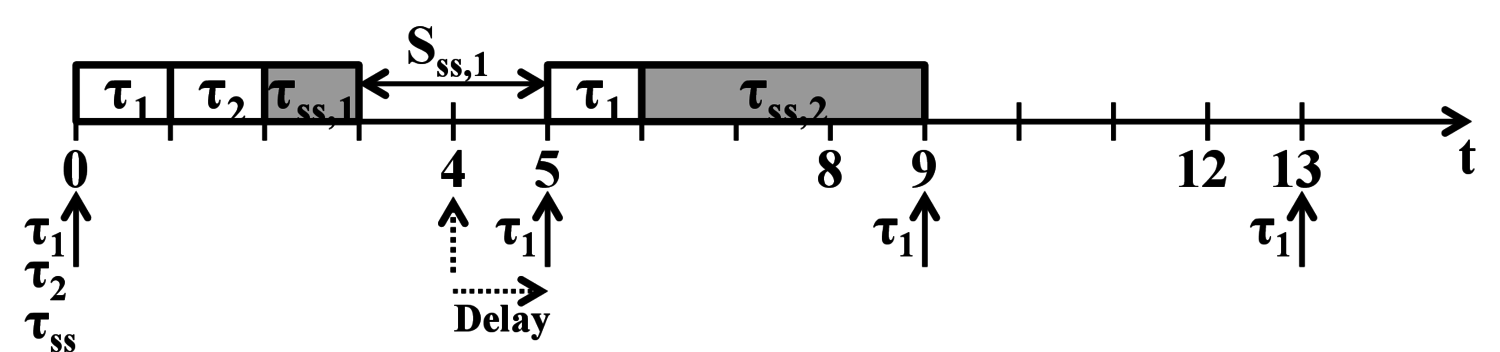
\includegraphics[width=0.85\linewidth]{ex-phi}} \\
  \subfloat[Worst-case response-time of $\tau_3$ when when all tasks do not release a job synchronously.]{\label{fig:ex-no-phi} 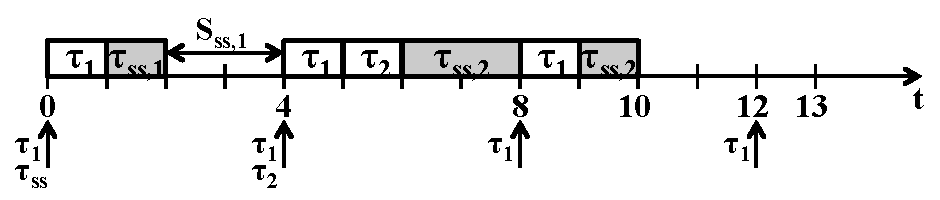
\includegraphics[width=0.85\linewidth]{ex-no-phi}}
  \caption{Counter-example to the synchronous release of all tasks.}
  \label{fig:ex-synch-releases}
\end{figure}

Consider three implicit deadline tasks with the parameters presented in Table~\ref{table:ex-synch-releases}. Let us assume that the priorities of the tasks are assigned using the rate monotonic policy (i.e., the smaller the period, the higher the priority). We are interested in computing the worst-case response time of $\tau_3$. Following the definition of the critical instant presented in \cite{RTAS-LakshmananR10}, all three tasks must release a job synchronously at time $0$. Using the standard response-time analysis for non-self-suspending tasks, we get that the worst-case response time of the first computation region of $\tau_3$ is equal to $R_3^1 = 3$. Because the second job of $\tau_1$ would be released in the self-suspending interval of $\tau_3$ if $\tau_1$ was strictly respecting its minimum inter-arrival time, the release of the second job of $\tau_1$ is delayed so as to coincide with the release of the second computation region of $\tau_3$ (see Figure~\ref{fig:ex-phi}). Considering the fact that the second job of $\tau_2$ cannot be released before time instant $50$ and hence does not interfere with the execution of $\tau_3$, the response time of the second computation segment of $\tau_3$ is thus equal to $R_3^2=4$. In total, the worst-case response time of $\tau_3$ when all tasks release a job synchronously is equal to 
$$R_3 = R_3^1 + S_3^2 + R_3^2 = 3 + 2 +4 = 9$$

Now, let us consider a job release pattern as shown in Figure~\ref{fig:ex-no-phi}. Task $\tau_2$ does not release a job synchronously with task $\tau_3$ but with its second computation segment instead. The response time of the first computation segment of $\tau_3$ is thus reduced to $R_3^1=2$. However, both $\tau_1$ and $\tau_2$ can now release a job synchronously with the second computation segment of $\tau_3$, for which the response time is now equal to $R_3^2=6$ (see Fig.~\ref{fig:ex-no-phi}). Thus, the total response time of $\tau_3$ in a scenario where not all higher priority tasks release a job synchronously with $\tau_3$ is equal to 
$$R_3 = R_3^1 + S_3^2 + R_3^2 = 2+2+6 = 10$$

To conclude, the synchronous release of all tasks does not necessarily generate the maximum interference for the self-suspending task $\tau_i$ and is thus not always a critical instant for $\tau_i$. It was however proven in \cite{ecrts15nelissen} that in the critical instant of a self-suspending task $\tau_i$, every higher priority task releases a job synchronously with the arrival of at least one computation segment of $\tau_i$, but not all higher priority tasks must release a job synchronously with the same computation segment.

\subsection{Incorrect Quantifications of Additional Interferences due to Carry-In Jobs}
\label{sec:wrong-carryin}

\subsection{Incorrect Quantifications of Jitter}
\label{sec:wrong-jitter}


\subsection{Incorrect Periodic Execution Enforcement}
\label{sec:wrong-periodic}


